\scanpage{372}\mspage{II}
\margin{Coh d'EM}
\deleted{\unsure{Th un|Th en} $\mathbb F_p$-modules}

Th (Cartan) : $G,H$ deux \deleted{anneaux} \inserted{groupes} (il fait des hyp sur $G$ et $H$),)
\[
H_*(K(G,n),H)\simeq H_*(K(H,n),G)\qquad\text{additif.}
\]
\uline{Dém} : Calcul.

\figure{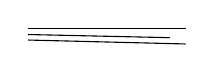
\begin{tikzpicture}\draw (0,0)--(2,0);\draw (0,-.08)--(1.8,-.12);\draw (0,-.15)--(2,-.2);\end{tikzpicture}}
$X$ un ensemble simplicial pointé.
\margin{$\pi_i(\mathbb ZX)=H_i(X)$}
\[
K(\mathbb Z,n)\wedge X\xrightarrow{A(X)}\deleted{\mathbb Z X}\mathbb Z^{+}(S^nX)
\]
\margin{$\mathbb Z^{+}(X,x)=\mathbb ZX/\mathbb Zx$}
$2n-1$ quasi isomorphisme.
\[
K(\mathbb Z,n)=\mathbb Z^{+}[S^n]
\]
\[
K(\mathbb Z,n)\wedge\underline X\longrightarrow K(\mathbb Z,n)\wedge\mathbb Z^+X
\]
\[
\left.\begin{aligned}
\mathbb Z\,X\times Y&\simeq\mathbb ZX\otimes\mathbb ZY\\
\mathbb Z^+(X\wedge Y)&\simeq\mathbb Z^+X\otimes\mathbb Z^+Y
\end{aligned}\right\}\quad
\begin{array}{l}EZ\\ EZ\ \text{pointé.}\end{array}
\]
\[
\mathbb Z^+(S^n)\wedge X\longrightarrow\mathbb Z^+(S^n)\wedge\mathbb Z^+X
\longrightarrow\mathbb Z^+(S^n)\otimes\mathbb Z^+X\xrightarrow{EZ}\mathbb Z^+(S^nX)
\]
\[
\pi_{n+r}(K(\mathbb Z,n)\wedge X)=\pi_{n+r}(\mathbb Z^+(S^nX))
=\widetilde H_{n+r}(S^nX)=\widetilde H_r(X)
\]
\uline{Dém} : $A(S^n)$
\[
\pi_i(K(\mathbb Z,n)\wedge S^m)\qquad
\mathbb Z^+(S^n\wedge S^m)=\mathbb Z^+(S^{n+m})
\]

\figure{\begin{tikzpicture}\node[inner sep=9pt] (box) {\begin{minipage}{.84\linewidth}
Ex de la dem 2 : interpretation du diagramme $(*)$ en bas de la page I
\diagram{\begin{tikzcd}[column sep=small,row sep=small]
K(\mathbb Z,n)\wedge K(\mathbb F_p,m)\arrow[r]\arrow[d,bend right=12]&
K(\mathbb F_p;m)\wedge K(\mathbb Z,n)\arrow[d]\\
K(\deleted{\mathbb Z}\mathbb F_p,n)\wedge K(\mathbb F_p,n)\arrow[r]&
K(\mathbb F_p,n)\wedge K(\mathbb F_p,n)
\end{tikzcd}}
\end{minipage}};\draw (box.north west) to[out=5,in=175] (box.north east) -- ([yshift=10pt]box.south east) to[out=-90,in=0] ([xshift=-24pt]box.south east) -- ([xshift=-24pt,yshift=-8pt]box.south east) to[out=200,in=0] ([yshift=-8pt]box.south west);\end{tikzpicture}}
\[
\begin{aligned}
S^m\wedge K(\mathbb Z,n)&\xrightarrow{\mathrm{qi}\ldots} K(\mathbb Z,n+m)\\
S^m&\longrightarrow\mathbb Z^+(S^m)=K(\mathbb Z,m)\\
S^m\wedge\deleted{K}K(\mathbb Z,n)&\longrightarrow K(\mathbb Z,m)\wedge K(\mathbb Z,n)\xrightarrow{\cup}K(\mathbb Z,n+m).
\end{aligned}
\]
Pt clef : $X\xrightarrow{h_r(\ )}\pi_{n+r}(K(\mathbb Z,n)\wedge X)$ est une th d'homologie partielle
\[
Y\hookrightarrow X\longrightarrow X/Y
\]
induit $h_r(Y)\longrightarrow h_r(X)\longrightarrow h_r(X/Y)\longrightarrow h_{r-1}(Y)\longrightarrow\ldots$

\uline{$r$ assez petit}.

Dem 2 du th de Cartan
\[
\pi_{i+m}(K(H,m)\wedge K(G,n)\simeq\pi_{i+n}(K(G,n)\wedge K(H,n))
\]
s'obtient par permutation des facteurs
\mspage{373}
